% ==============================================================
%  MEMORIA TFG — Tipo II
%  Diseño y Desarrollo de una Plataforma Software para la
%  Optimización de Comunidades Energéticas
%
%  Alumno : Roberto Rodríguez Núñez
%  Titora : Eva Mª Lorenzo Iglesias
%  Cotitor: Pedro Celard Pérez
%  Centro : ESEI — Universidade de Vigo  |  Curso 2024/2025
% ==============================================================

\documentclass[12pt, a4paper, twoside]{report}

\usepackage[utf8]{inputenc}
\usepackage[T1]{fontenc}
\usepackage[spanish]{babel}
\usepackage{amsmath, amssymb}
\usepackage{siunitx}
\sisetup{output-decimal-marker={,}, group-separator={.}}
\usepackage{microtype}
\usepackage[top=2.5cm, bottom=2.5cm, inner=3cm, outer=2.5cm]{geometry}
\usepackage{setspace}
\onehalfspacing
\usepackage{parskip}
\setlength{\parindent}{0pt}
\setlength{\parskip}{6pt plus 2pt minus 1pt}

\usepackage{fancyhdr}
\pagestyle{fancy}
\fancyhf{}
\fancyhead[LE,RO]{\small\thepage}
\fancyhead[RE]{\small\nouppercase{\leftmark}}
\fancyhead[LO]{\small\nouppercase{\rightmark}}
\renewcommand{\headrulewidth}{0.4pt}
\fancypagestyle{plain}{
  \fancyhf{}
  \fancyfoot[C]{\small\thepage}
  \renewcommand{\headrulewidth}{0pt}
}

\usepackage{titlesec}
\titleformat{\chapter}[display]
  {\normalfont\Large\bfseries}
  {\chaptertitlename\ \thechapter}{16pt}{\Huge}
\titlespacing*{\chapter}{0pt}{-10pt}{30pt}

\usepackage{booktabs, array, longtable, tabularx}
\newcolumntype{L}[1]{>{\raggedright\arraybackslash}p{#1}}
\newcolumntype{C}[1]{>{\centering\arraybackslash}p{#1}}
\usepackage{graphicx, caption, subcaption, float}
\usepackage{enumitem}
\usepackage{tocloft}
\renewcommand{\cftchapfont}{\bfseries}
\renewcommand{\cftchappagefont}{\bfseries}
\setlength{\cftbeforechapskip}{6pt}

\usepackage{xcolor}
\definecolor{codebg}{RGB}{248,248,248}
\definecolor{codeframe}{RGB}{210,210,210}
\definecolor{kw}{RGB}{0,0,180}
\definecolor{cmt}{RGB}{100,100,100}
\definecolor{str}{RGB}{163,21,21}
\usepackage{listings}
\lstset{
  backgroundcolor=\color{codebg}, frame=single,
  rulecolor=\color{codeframe},
  basicstyle=\small\ttfamily,
  keywordstyle=\color{kw}\bfseries,
  commentstyle=\color{cmt}\itshape,
  stringstyle=\color{str},
  breaklines=true, captionpos=b,
  numbers=left, numberstyle=\tiny\color{gray},
  numbersep=8pt, showstringspaces=false,
  xleftmargin=15pt, language=Python
}

\usepackage[hidelinks, breaklinks=true]{hyperref}
\usepackage{pdfpages}
\usepackage{cleveref}
\usepackage{natbib}
\bibliographystyle{plainnat}

\usepackage[acronym, toc, nonumberlist]{glossaries}
\makeglossaries
\newacronym{rl}{RL}{Aprendizaje por Refuerzo (\textit{Reinforcement Learning})}
\newacronym{sac}{SAC}{Soft Actor-Critic}
\newacronym{dqn}{DQN}{Deep Q-Network}
\newacronym{ppo}{PPO}{Proximal Policy Optimization}
\newacronym{td3}{TD3}{Twin Delayed Deep Deterministic Policy Gradient}
\newacronym{ddpg}{DDPG}{Deep Deterministic Policy Gradient}
\newacronym{mpc}{MPC}{Control Predictivo Basado en Modelos}
\newacronym{lp}{LP}{Programación Lineal}
\newacronym{ems}{EMS}{Sistema de Gestión Energética}
\newacronym{bess}{BESS}{Sistema de Almacenamiento de Energía en Baterías}
\newacronym{lfp}{LFP}{Litio Hierro Fosfato}
\newacronym{pvpc}{PVPC}{Precio Voluntario para el Pequeño Consumidor}
\newacronym{soc}{SoC}{Estado de Carga}
\newacronym{etl}{ETL}{Extracción, Transformación y Carga}
\newacronym{api}{API}{Interfaz de Programación de Aplicaciones}
\newacronym{ccee}{CCEE}{Comunidad Energética de Autoconsumo}
\newacronym{fv}{FV}{Fotovoltaico}
\newacronym{mdp}{MDP}{Proceso de Decisión de Markov}
\newacronym{sb3}{SB3}{Stable-Baselines3}
\newacronym{saas}{SaaS}{Software como Servicio}
\newacronym{mer}{MER}{Modelo Entidad-Relación}

\hypersetup{
  pdftitle={Diseño y Desarrollo de una Plataforma Software para la Optimización de Comunidades Energéticas},
  pdfauthor={Roberto Rodríguez Núñez},
  pdfsubject={TFG Tipo II — ESEI, Universidade de Vigo, 2025}
}

% ==============================================================
\begin{document}
% ==============================================================

% ── PORTADA OFICIAL ───────────────────────────────────────────
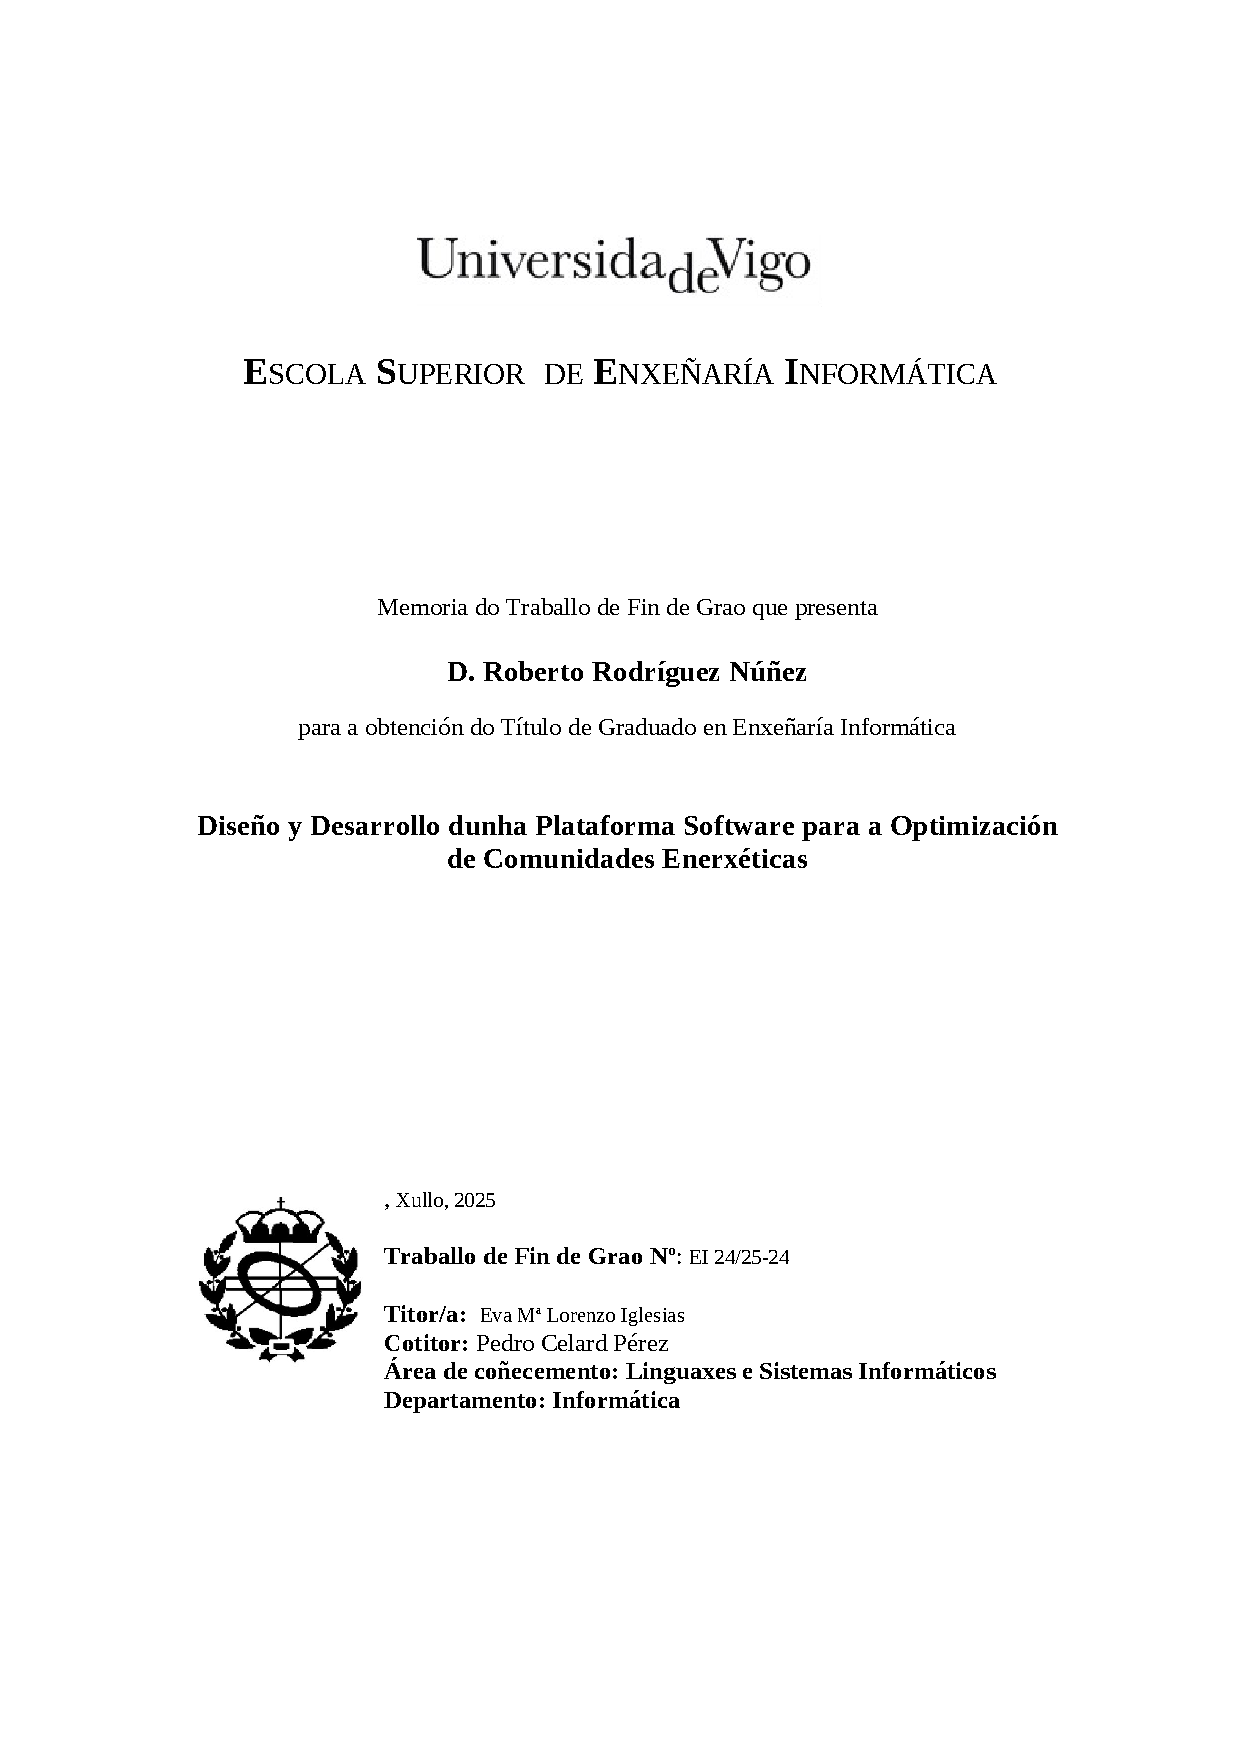
\includepdf[pages=1, fitpaper=true]{portada_oficial}

% ── PRELIMINARES ──────────────────────────────────────────────
\pagenumbering{roman}
\setcounter{page}{1}

\chapter*{Dedicatoria}
\addcontentsline{toc}{chapter}{Dedicatoria}
\thispagestyle{plain}
\vspace*{4cm}
\begin{flushright}\textit{[Espacio reservado]}\end{flushright}

\chapter*{Agradecimientos}
\addcontentsline{toc}{chapter}{Agradecimientos}
\thispagestyle{plain}
[Espacio reservado para agradecimientos]

% ── Resumen ───────────────────────────────────────────────────
\chapter*{Resumen}
\addcontentsline{toc}{chapter}{Resumen}
\thispagestyle{plain}

El actual marco regulatorio del autoconsumo colectivo en España, consolidado
mediante el Real Decreto 244/2019, ha abierto una oportunidad para que las
comunidades de pequeña escala gestionen de forma autónoma su energía
fotovoltaica. Sin embargo, las soluciones de gestión inteligente disponibles se
orientan al almacenamiento individual o industrial y suelen ser cerradas y
propietarias, lo que dificulta su adaptación a la batería compartida de una
comunidad, el activo más valioso de la instalación.

Este trabajo investiga, diseña e implementa un motor de decisión inteligente
basado en aprendizaje por refuerzo para la optimización económica de la batería
comunitaria en una comunidad energética de autoconsumo fotovoltaico colectivo.
Tras un proceso documentado de experimentación con los algoritmos \acrshort{dqn}
y \acrshort{ppo}, se diseña e implementa el controlador Residual \acrshort{sac}
sobre un \acrshort{mpc} base, arquitectura híbrida que resuelve los problemas de
arranque en frío y cuantización que impidieron a los candidatos anteriores
superar el \textit{baseline} competitivo de $+48{,}73$\,€/semana.

El motor se integra en una plataforma software de tipo \acrshort{saas} con
gemelo digital de la instalación, módulo de ingeniería de datos con fuentes
oficiales (ESIOS, PVGIS) y capa de visualización diferenciada por rol
(Administrador y Vecino de la comunidad). El sistema implementa la capa de
planificación horaria (Nivel~3) del control jerárquico estándar para sistemas
de almacenamiento, replicando la lógica de despacho horario utilizada por
los agregadores energéticos en el mercado diario de OMIE.

\textbf{Palabras clave:} comunidades energéticas, autoconsumo colectivo,
aprendizaje por refuerzo, Soft Actor-Critic, control predictivo basado en
modelos, RD 244/2019, optimización energética.

\chapter*{Abstract}
\addcontentsline{toc}{chapter}{Abstract}
\thispagestyle{plain}

Spain's regulatory framework for collective self-consumption, established by
Royal Decree 244/2019, has created an opportunity for small-scale communities
to autonomously manage their photovoltaic energy. However, the lack of
accessible tools forces reliance on static sharing models that underutilise
the installation's most valuable asset: the community battery.

This work investigates, designs and implements an intelligent decision engine
based on reinforcement learning for the economic optimisation of the community
battery in a collective photovoltaic self-consumption energy community. After
a documented experimentation process with DQN and PPO, the Residual SAC
controller over an MPC base is designed and implemented, a hybrid architecture
that resolves the cold-start and quantisation problems that prevented previous
candidates from surpassing the competitive baseline of
$+51.69 \pm 30.21$\,€/week.

\textbf{Keywords:} energy communities, collective self-consumption,
reinforcement learning, Soft Actor-Critic, model predictive control,
RD 244/2019.

\tableofcontents
\listoffigures
\addcontentsline{toc}{chapter}{Índice de figuras}
\listoftables
\addcontentsline{toc}{chapter}{Índice de tablas}
\printglossary[type=acronym, title={Glosario de Acrónimos}]

% ── CUERPO ────────────────────────────────────────────────────
\pagenumbering{arabic}
\setcounter{page}{1}

% ==============================================================
\chapter{Introducción}
\label{chap:intro}
% ==============================================================

\section{Contexto y Problemática}

La transición energética hacia un modelo descarbonizado sitúa al autoconsumo
fotovoltaico colectivo como uno de los instrumentos más prometedores para
democratizar la generación de energía renovable a nivel ciudadano. El Real
Decreto 244/2019 consolidó en España el marco regulatorio que permite a varias
unidades de consumo compartir una instalación de generación fotovoltaica y
distribuir los excedentes entre sus participantes mediante coeficientes de
reparto horarios. Este mecanismo abre la puerta a un modelo energético más
justo y autónomo, especialmente en el entorno rural.

Sin embargo, la puesta en práctica de este potencial choca con una realidad
técnica: las soluciones de gestión energética inteligente disponibles se
orientan sobre todo al almacenamiento individual o industrial, donde la batería
responde a un único punto de consumo, y suelen ser cerradas y propietarias. La
batería de una comunidad de autoconsumo colectivo plantea un problema distinto,
pues un único activo debe gestionarse de forma centralizada para el balance
agregado de todos los participantes, y queda infrautilizada sin una política de
carga y descarga que explote la variabilidad horaria del precio de la energía
en el mercado español.

La variabilidad del precio PVPC, que en 2022 alcanzó \SI{0,50}{€/kWh} en horas
pico y valores cercanos a cero en horas valle, ofrece un margen de arbitraje
que solo un motor de decisión con capacidad predictiva puede explotar. El
presente trabajo aborda este problema desde una perspectiva dual: investigadora,
al desarrollar y comparar algoritmos de aprendizaje por refuerzo aplicados a
este dominio; e ingenieril, al integrar el motor resultante en una plataforma
software accesible para comunidades rurales de pequeña escala.

\section{Posicionamiento en el Control Jerárquico Estándar}

El sistema implementa la \textbf{capa de planificación horaria (Nivel~3)} del
control jerárquico estándar para sistemas de almacenamiento de energía. Esta
capa opera con horizonte de 24 horas y resolución horaria, determinando la
estrategia económicamente óptima de carga y descarga en función del pronóstico
de precios, generación y consumo. La integración con la capa de control
supervisorio (Nivel~2, SCADA) y la capa de control en tiempo real (Nivel~1,
BMS) queda como trabajo futuro para el despliegue en instalaciones reales.

Desde la perspectiva del mercado eléctrico, la arquitectura replica la capa de
despacho horario utilizada por los agregadores energéticos en el mercado diario
español (OMIE). La participación en mercados intradiarios de OMIE y en servicios
de balance de REE —que operan en horizontes sub-horarios— queda como extensión
natural hacia una arquitectura de gestión energética multi-capa completa.

\section{Estructura del Documento}

El documento sigue la estructura del Tipo~II de la Guía de Elaboración del TFG
de la ESEI. El Capítulo~\ref{chap:objetivos} define los objetivos. El
Capítulo~\ref{chap:antecedentes} revisa los antecedentes y el contexto del
problema. El Capítulo~\ref{chap:solucion} resume la solución propuesta y
la metodología. El Capítulo~\ref{chap:marco} desarrolla el marco teórico y
las herramientas empleadas, constituyendo junto con los capítulos siguientes
el núcleo técnico del trabajo. El Capítulo~\ref{chap:datos} describe la
ingeniería de datos y el gemelo digital físico-económico de la comunidad.
El Capítulo~\ref{chap:motor} desarrolla el motor de decisión en profundidad.
Los Capítulos~\ref{chap:planificacion} a~\ref{chap:futuro} completan la
documentación con planificación, aportaciones, conclusiones y trabajo futuro.

% ==============================================================
\chapter{Objetivos}
\label{chap:objetivos}
% ==============================================================

El objetivo central del presente trabajo es el diseño, implementación y
validación experimental de un motor de decisión basado en aprendizaje por
refuerzo para la optimización económica de la batería comunitaria en una
comunidad energética de autoconsumo fotovoltaico colectivo, operando bajo el
marco regulatorio del RD 244/2019, e integrado en una plataforma software
accesible orientada a comunidades rurales de pequeña escala.

\section{Objetivos Generales}

\begin{enumerate}[label=\textbf{OG\arabic*.}]
  \item Investigar y comparar algoritmos de aprendizaje por refuerzo aplicados
    a la gestión de sistemas de almacenamiento de energía, con especial atención
    a su capacidad para superar un \textit{baseline} de control predictivo bien
    calibrado.
  \item Diseñar e implementar un gemelo digital físico-económico de una comunidad
    energética, calibrado con datos reales de fuentes oficiales (ESIOS, PVGIS),
    que sirva como entorno de entrenamiento y evaluación reproducible.
  \item Seleccionar, justificar e implementar el algoritmo de control más adecuado
    tras experimentación documentada con candidatos alternativos.
  \item Integrar el motor de decisión en una plataforma software accesible que
    democratice la gestión energética inteligente para comunidades rurales.
\end{enumerate}

\section{Objetivos Específicos}

\begin{enumerate}[label=\textbf{OE\arabic*.}]
  \item Construir el pipeline \acrshort{etl} reproducible que integre datos de
    consumo normativo (ESIOS 2.0TD), generación \acrshort{fv} (PVGIS) y precios
    de mercado (PVPC e indicador de compensación simplificada) en un dataset
    unificado de 22.646 horas.
  \item Implementar el simulador físico-económico con modelo de degradación no
    lineal de batería LFP y modelo económico asimétrico coherente con el
    RD 244/2019.
  \item Implementar el controlador \acrshort{mpc} con horizonte deslizante de
    24 horas como cota teórica (pronóstico oráculo) y como \textit{baseline}
    competitivo (pronóstico realista con ruido AR(1)).
  \item Experimentar con \acrshort{dqn} y \acrshort{ppo} como algoritmos
    candidatos, documentando su rendimiento y sus limitaciones estructurales.
  \item Diseñar e implementar el controlador Residual \acrshort{sac} con
    protocolo de inicialización con demostraciones del MPC, y validar
    experimentalmente que supera al \textit{baseline} competitivo.
  \item Desarrollar una suite de tests automatizados que garantice los
    invariantes físicos y económicos del simulador y la reproducibilidad
    de los experimentos.
\end{enumerate}

\section{Alcance}

El trabajo cubre el diseño, implementación y validación experimental del motor
de decisión sobre datos históricos simulados. La integración con APIs de datos
en tiempo real está diseñada e implementada pero no activada en el prototipo
actual. El despliegue en hardware físico y la integración con datos de viviendas
reales constituyen extensiones naturales en el trabajo futuro.

% ==============================================================
\chapter{Antecedentes y Contexto}
\label{chap:antecedentes}
% ==============================================================

\section{Marco Regulatorio del Autoconsumo Colectivo en España}

El autoconsumo colectivo en España, en transposición de la normativa europea
sobre energías renovables y mercado interior de la electricidad, se regula
mediante el \textbf{Real Decreto 244/2019}, que establece las condiciones
administrativas, técnicas y económicas del autoconsumo e introduce el mecanismo
de \textbf{compensación simplificada de excedentes}, posteriormente reforzado
por el Real Decreto-ley 7/2025.

El mecanismo realiza una liquidación económica hora a hora del intercambio de
energía entre la comunidad y la red. En cada hora se compara la generación
fotovoltaica total con el consumo total de la comunidad, y pueden darse dos
situaciones. Si la generación es \textbf{menor} que el consumo, la comunidad
autoconsume toda la energía solar producida (que no se factura, pues sustituye
energía que habría que comprar) y adquiere de la red el déficit restante al
precio de compra PVPC. Si la generación es \textbf{mayor} que el consumo, la
comunidad autoconsume la parte que cubre su demanda y vierte el excedente
sobrante a la red, recibiendo por él una compensación al precio mayorista.

Al final del periodo de facturación, la compensación acumulada por los
excedentes vertidos se descuenta del importe de la energía comprada. Esta
compensación está limitada: puede reducir la factura hasta cero, pero nunca
generar un saldo a favor del consumidor. La energía entra y sale físicamente de
la red con normalidad en ambas direcciones; el mecanismo de compensación es
únicamente la liquidación económica de ese intercambio.

Esta estructura justifica que el simulador modele la comunidad como
\textbf{nodo agregado}: lo que se liquida es el balance horario entre el consumo
y la generación totales de la comunidad, no el detalle vivienda a vivienda. La
característica que condiciona el diseño del motor de decisión es la asimetría de
precios: el precio de venta de excedentes (mayorista, indicador 1739 de ESIOS)
es sistemáticamente inferior al de compra (PVPC, indicador 1001), que incluye
peajes y cargos del sistema. Por ello, maximizar el autoconsumo interno es
siempre más rentable que maximizar la venta de excedentes.

\section{El Problema de la Gestión de Baterías en Comunidades Energéticas}

La inclusión de un sistema de almacenamiento de energía en baterías
(\acrshort{bess}) en una comunidad de autoconsumo introduce un problema de
decisión secuencial bajo incertidumbre: en cada hora del día, el gestor debe
decidir cuánta energía cargar o descargar de la batería considerando el precio
actual de la energía, la generación solar disponible, el consumo esperado de
las viviendas y el estado de carga actual de la batería.

Este problema tiene tres características que lo hacen especialmente adecuado
para técnicas de optimización avanzada. En primer lugar, las decisiones son
secuencialmente dependientes: cargar la batería ahora reduce el margen de carga
disponible en las próximas horas. En segundo lugar, existe incertidumbre sobre
el futuro: ni el consumo, ni la generación solar, ni siquiera el precio de la
energía son perfectamente predecibles con horas de antelación. En tercer lugar,
el horizonte de decisión relevante es de 24 horas, suficiente para que el precio
varíe entre máximos y mínimos que crean oportunidades de arbitraje temporal. El
precio, además, solo se conoce con exactitud de forma parcial: REE publica el
\acrshort{pvpc} del día siguiente a partir de las 20:00\,h, de modo que dentro
del horizonte de 24 horas las primeras horas son ciertas y las posteriores deben
estimarse, diferencia que motiva el modelo de pronóstico en tres capas empleado
en este trabajo (Capítulo~\ref{chap:motor}).

La estrategia realmente óptima no es evidente a priori: depende de la
interacción entre generación, consumo, precio y degradación, todos ellos
sujetos a incertidumbre dentro del horizonte de 24 horas, y es precisamente lo
que el motor de decisión debe aprender o calcular.

\section{El Espacio de Acciones: Discreto frente a Continuo}

La aplicación de aprendizaje por refuerzo a la gestión de sistemas de
almacenamiento de energía ha experimentado un crecimiento notable en la última
década, desde los trabajos fundacionales de \citet{Mnih2015} sobre
\acrshort{dqn}. La decisión de diseño más determinante en este dominio es la
topología del espacio de acciones, que condiciona estructuralmente tanto el
algoritmo aplicable como la calidad de la política aprendida.

Un \textbf{espacio discreto} representa las decisiones de la batería como un
conjunto finito de acciones que combinan estrategia (cargar, descargar, no
actuar) con nivel de potencia. Es la representación que emplean algoritmos
basados en valor como \acrshort{dqn}, y encaja bien con la gestión eléctrica
porque la estrategia rentable suele consistir en concentrar la carga y la
descarga en los picos y valles de precio, que son decisiones de naturaleza
discreta. Su ventaja es la simplicidad y la estabilidad de entrenamiento. Su
limitación es el error de cuantización: el conjunto finito de niveles no puede
representar los ajustes de potencia intermedios que la política óptima requiere
en algunas horas. En este trabajo se experimentó con \acrshort{dqn} y también
con \acrshort{ppo} sobre el mismo espacio discreto.

Un \textbf{espacio continuo} asigna directamente la potencia neta dentro del
rango físico del inversor. Elimina por construcción el error de cuantización a
costa de requerir algoritmos de control continuo más sofisticados como
\acrshort{sac}.

\section{Estado del Arte: RL puro frente a MPC y la Arquitectura Híbrida}

La comparativa honesta del RL con controladores \acrshort{mpc} bien calibrados
muestra un panorama matizado. En el contexto regulatorio español del PVPC, un
MPC determinista correctamente sintonizado captura ya en torno al 90\,\% del
valor económico disponible mediante arbitraje diario y emparejamiento de picos
de precio. La literatura sobre arquitecturas residuales en dominios afines
(microrredes, sistemas HVAC) documenta que el margen de mejora realista que un
esquema híbrido puede aportar sobre ese MPC se sitúa típicamente entre el 4\,\%
y el 12\,\%, reduciéndose a valores más modestos cuando el MPC ya está bien
calibrado. Este margen acotado, lejos de invalidar el enfoque, define con
precisión el espacio en el que el motor de IA debe demostrar su valor.

La arquitectura híbrida MPC+RL responde a esta realidad combinando la
estabilidad y las garantías del MPC con la capacidad adaptativa del RL.
\citet{Johannink2019} propusieron el \textit{Residual Reinforcement Learning}
en el contexto del control robótico: el agente aprende únicamente las
correcciones residuales sobre un controlador base competente, aprovechando el
conocimiento encapsulado en ese controlador como punto de partida. Aplicada al
presente trabajo, esta arquitectura aporta una propiedad de \textbf{seguridad
por construcción}: como la corrección del agente está acotada, si el agente
propone una corrección nula el sistema replica exactamente el comportamiento
del MPC subyacente, eliminando el riesgo de exploración destructiva que
desaconseja el uso de RL puro en infraestructuras críticas.

La selección del algoritmo de RL continuo para calcular la corrección residual
se desarrolla en detalle en el Capítulo~\ref{chap:motor}, donde se justifica la
elección de \acrshort{sac} frente a las alternativas continuas (PPO, TD3, DDPG)
sobre la base de su eficiencia de muestreo y su robustez ante la alta varianza
de la recompensa económica.

\section{Soluciones Actuales para la Gestión del Almacenamiento}

La gestión de baterías con inteligencia artificial es ya una realidad, tanto en
el ámbito comercial como en proyectos de investigación. Las soluciones
existentes se orientan sobre todo al almacenamiento individual o industrial,
donde la batería responde a un único punto de consumo, y suelen ser de carácter
cerrado y propietario. Esto las hace difíciles de auditar y de adaptar a
contextos para los que no fueron diseñadas, especialmente en comunidades de
pequeña escala con recursos limitados.

La batería de una comunidad de autoconsumo colectivo plantea un problema
distinto, porque un único activo debe gestionarse de forma centralizada para el
balance agregado de todos los participantes bajo el marco del RD 244/2019. La
energía generada se reparte entre las viviendas y solo el excedente conjunto se
vierte a la red, de modo que la decisión de carga y descarga afecta a toda la
comunidad y no a un consumidor aislado. El presente trabajo se centra en este
escenario, aplicando aprendizaje por refuerzo a la optimización económica del
almacenamiento comunitario y midiendo de forma transparente la mejora que aporta
frente a un control de referencia bien calibrado.

% ==============================================================
\chapter{Resumen de la Solución Propuesta y Metodología}
\label{chap:solucion}
% ==============================================================

\section{Descripción General}

La solución propuesta es la plataforma EnergyComm, un sistema software que
implementa un gemelo digital de una comunidad energética de autoconsumo
fotovoltaico colectivo y un motor de decisión basado en aprendizaje por
refuerzo para la optimización económica de la batería comunitaria. La comunidad
simulada comprende quince viviendas con perfil de consumo residencial 2.0TD,
una instalación fotovoltaica compartida de \SI{50}{kWp} y una batería
comunitaria de tecnología \acrshort{lfp} con capacidad de \SI{100}{kWh} e
inversor bidireccional de \SI{50}{kW}.

La plataforma se organiza en cinco capas funcionales. La \textbf{capa de datos}
construye y mantiene el dataset de simulación a partir de fuentes oficiales. La
\textbf{capa del simulador} implementa el gemelo digital físico-económico. La
\textbf{capa de aprendizaje por refuerzo} contiene el entorno Gymnasium y el
motor de decisión. La \textbf{capa de producción} gestiona el ciclo de vida del
modelo entrenado y su exportación a formato ONNX para despliegue en hardware de
borde. La \textbf{capa SaaS} expone los resultados a los usuarios finales a
través de dashboards Streamlit diferenciados por rol, con persistencia en
PostgreSQL.

\begin{figure}[H]
  \centering
  \fbox{\parbox{0.92\textwidth}{\centering\vspace{3cm}
    \textit{[Figura: Arquitectura de 5 capas de la plataforma EnergyComm]}\\
    \textit{Exportar arquitectura\_capas.drawio $\rightarrow$ img/arquitectura\_capas.png}
  \vspace{3cm}}}
  \caption{Arquitectura de la plataforma EnergyComm organizada en cinco capas.}
  \label{fig:arquitectura}
\end{figure}

\section{Metodología}

El desarrollo sigue un ciclo iterativo de tipo Scrum con sprints semanales,
adaptado a las características de un proyecto de investigación aplicada. Las
iteraciones alternan entre el desarrollo de componentes software y la
experimentación con el motor de decisión, con validación continua mediante la
suite de tests automatizados.

Se aplica la metodología MLOps al ciclo de vida del motor de decisión:
configuración externalizada en YAML (sin \textit{magic numbers} en el código),
semillas fijas para reproducibilidad total de experimentos, versionado de modelos
entrenados y de las estadísticas de normalización (\texttt{vec\_normalize.pkl}),
y trazabilidad de curvas de entrenamiento mediante TensorBoard.

El proceso de selección del algoritmo final siguió un protocolo de
experimentación estructurado: establecimiento de cotas de rendimiento mediante
MPC, experimentación con candidatos (DQN, PPO) con análisis de limitaciones, y
diseño del controlador final (Residual SAC) que resuelve esas limitaciones. Este
protocolo garantiza que la selección del algoritmo está basada en evidencia
experimental y no en preferencias a priori.

% ==============================================================
\chapter{Marco Teórico y Herramientas Empleadas}
\label{chap:marco}
% ==============================================================

\section{Fundamentos del Aprendizaje por Refuerzo}
\label{sec:fundamentos_rl}

\subsection{Proceso de Decisión de Markov}

El problema de gestión de la batería comunitaria se formula como un
\acrfull{mdp} definido por la tupla $(\mathcal{S}, \mathcal{A}, P, R, \gamma)$.
El espacio de estados $\mathcal{S}$ recoge las variables observables en cada
paso temporal $h$: el estado de carga $\text{SoC}_h \in [0{,}10, 0{,}90]$, el
precio de compra $p_c^h$, el precio de venta $p_v^h$, el excedente solar
$e_h = \max(0, g_h - c_h)$ y el déficit de consumo $d_h = \max(0, c_h - g_h)$.

El espacio de acciones $\mathcal{A}$ define los flujos energéticos que el
controlador puede modular en cada hora: energía solar cargada en batería $c_s$,
energía de red cargada en batería $c_m$, energía descargada para consumo $d_c$
y energía descargada vendida a red $d_r$. Estos cuatro flujos están acoplados
por las restricciones físicas del sistema.

La función de recompensa $R(s,a)$ es el beneficio marginal respecto a la
política de referencia IDLE (batería desconectada):
\begin{equation}
  r_h = E_{\text{vend},h}\,p_v^h - E_{\text{comp},h}\,p_c^h - c_{\text{deg},h}
  \label{eq:recompensa}
\end{equation}

El factor de descuento $\gamma = 0{,}99$ establece un horizonte efectivo de
$1/(1-\gamma) = 100$ pasos, equivalente a unos cuatro días dentro de los
episodios semanales de 168 horas. Esto garantiza que el agente pondere las
consecuencias de sus decisiones sobre el estado de carga más allá del horizonte
de planificación de 24 horas, valorando el efecto de cargar o descargar la
batería sobre las jornadas siguientes.

\subsection{Familias de Algoritmos Aplicables}

Los algoritmos de \acrshort{rl} para control continuo se organizan en tres
familias. Los métodos \textit{value-based} (DQN y variantes) requieren espacio
de acción discreto y aprenden $Q(s,a;\theta)$. Los métodos
\textit{policy gradient on-policy} (PPO, A3C) aprenden directamente la política
$\pi_\theta(a|s)$ actualizando con trayectorias del agente actual. Los métodos
\textit{actor-critic off-policy} (SAC, TD3) combinan actor y crítico con
\textit{replay buffer}, siendo más eficientes en muestras y adecuados para
espacios de acción continuos.

\subsection{Soft Actor-Critic}

El algoritmo \acrfull{sac} \citep{Haarnoja2018} incorpora un término de entropía
máxima en el objetivo de aprendizaje:
\begin{equation}
  \pi^* = \arg\max_\pi \sum_t \mathbb{E}_{(s_t,a_t)\sim\pi}\!\left[
    r(s_t,a_t) + \alpha\,\mathcal{H}(\pi(\cdot|s_t))
  \right]
  \label{eq:sac_objetivo}
\end{equation}

donde $\mathcal{H}(\pi(\cdot|s_t))$ es la entropía de la política en el estado
$s_t$ y $\alpha$ es el coeficiente de temperatura. Este término de entropía
regula automáticamente la exploración: cuando la política es determinista
(baja entropía), el agente explora más; cuando es estocástica (alta entropía),
el agente explota el conocimiento actual. Esta propiedad proporciona una
robustez notable a hiperparámetros, siendo SAC la elección preferida en
aplicaciones de control continuo con restricciones físicas.

\section{Control Predictivo Basado en Modelos (MPC)}
\label{sec:mpc_teoria}

El \acrfull{mpc} es un paradigma de control óptimo que resuelve en cada paso
temporal un problema de optimización de horizonte finito, aplicando solo la
primera acción de la secuencia óptima y repitiendo el proceso en el siguiente
paso \citep{Rawlings2017}. En el contexto de la gestión energética, el MPC
con horizonte de 24 horas determina el perfil óptimo de carga y descarga para
las próximas 24 horas, ejecuta la decisión de la hora actual, y recalcula con
la información actualizada.

La principal ventaja del MPC es que puede incorporar explícitamente las
restricciones físicas del sistema (límites de SoC, potencia máxima) y optimizar
una función objetivo económica bien definida. Su principal limitación es que
su rendimiento depende de la calidad del modelo del sistema y del pronóstico
de las variables futuras.

\section{Arquitectura Residual MPC+RL}
\label{sec:residual_teoria}

La arquitectura Residual \acrshort{rl} \citep{Johannink2019} combina un
controlador base competente con un agente de RL que aprende únicamente las
correcciones residuales. La acción final es:
\begin{equation}
  a_{\text{final}} = \text{clip}\!\left(
    a_{\text{base}} + \Delta a \cdot \delta_{\max},\;
    \text{límites físicos}
  \right)
  \label{eq:residual_general}
\end{equation}

Con $\Delta a = \mathbf{0}$, el sistema es exactamente el controlador base.
El agente SAC solo necesita aprender en el espacio residual: las correcciones
sobre lo que el MPC ya hace bien. Esto resuelve la \textit{cold-start pathology}
pre-llenando el \textit{replay buffer} con demostraciones del controlador base.

\section{Herramientas y Stack Tecnológico}
\label{sec:herramientas}

\begin{table}[H]
\centering
\caption{Stack tecnológico de la plataforma EnergyComm.}
\label{tab:stack}
\begin{tabularx}{\textwidth}{lll}
\toprule
\textbf{Capa} & \textbf{Tecnología} & \textbf{Versión / Justificación} \\
\midrule
Lenguaje & Python & 3.11 — ecosistema ML estándar \\
Framework RL & Stable-Baselines3 & 2.3 — SAC, PPO, DQN auditados \\
Deep Learning & PyTorch & 2.2 — backend de SB3 \\
Entorno RL & Gymnasium (Farama) & 0.29 — estándar de facto \\
Optimización LP & SciPy / HiGHS & 1.12 — solver LP, optimalidad global \\
Datos & Pandas / NumPy & 2.x / 1.26 \\
Fuente precios & ESIOS API (REE) & Indicadores 1001 y 1739 \\
Fuente generación & PVGIS API (JRC-EU) & Producción FV histórica \\
Fuente previsión & Open-Meteo API & Irradiancia solar horaria \\
Runtime edge & ONNX Runtime & Inferencia sin SB3 ni Gymnasium \\
Base de datos & PostgreSQL & Perfiles, histórico, coeficientes \\
Frontend & Streamlit & Dashboard Admin + Dashboard Vecino \\
Configuración & YAML / OmegaConf & Hiperparámetros externalizados \\
Tracking ML & TensorBoard & Curvas entrenamiento y diagnóstico \\
Testing & pytest & 7.x — 19 tests automatizados \\
Control versiones & Git & Seeds, modelos, vec\_normalize \\
\bottomrule
\end{tabularx}
\end{table}

La selección de \acrshort{sb3} frente a RLlib se justifica por sus
implementaciones auditadas con verificación estática de tipos y soporte nativo
para \texttt{VecNormalize} y buffers de demostración, requisitos del protocolo
de inicialización con demostraciones del MPC. HiGHS garantiza optimalidad global
en el LP del MPC y detección explícita de infactibilidad, verificada sobre 1.000
escenarios aleatorios. La arquitectura de exportación a ONNX permite desplegar
el modelo entrenado en hardware de borde sin el stack completo de entrenamiento.

% ==============================================================
\chapter{Ingeniería de Datos y Entorno de Simulación}
\label{chap:datos}
% ==============================================================

\section{Fuentes de Datos Oficiales}

El dataset de simulación integra cuatro ficheros procedentes de tres fuentes
oficiales. El \textbf{perfil de consumo 2.0TD} (\texttt{consumo\_esios\_2021\_%
2023.csv}) se obtiene del indicador 808 de ESIOS, que publica coeficientes
horarios normalizados del consumo residencial elaborados a partir de medidas
reales de contadores inteligentes de la red española. Se escala a
$15 \times \SI{3500}{kWh/año} = \SI{52500}{kWh/año}$.

La \textbf{generación fotovoltaica} (\texttt{solar\_pvgis\_2021\_2023.csv})
procede de PVGIS (JRC-EU), que proporciona la producción unitaria horaria para
\SI{1}{kWp} en las coordenadas de la comunidad. Se escala a los \SI{50}{kWp}
de la instalación comunitaria aplicando un factor de pérdidas de sistema del
14\,\% (temperatura, suciedad, cableado e inversor).

Los \textbf{precios del mercado} se obtienen de dos indicadores de ESIOS:
el indicador 1001 (PVPC en €/MWh, fichero \texttt{precios\_esios\_2021\_2023.csv})
como precio de compra, y el indicador 1739 (compensación simplificada en €/MWh,
fichero \texttt{compensacion\_autoconsumo\_esios\_2021\_{...}.csv}) como precio
de venta de excedentes.

\section{Pipeline ETL}

El módulo \texttt{src/utils/generar\_dataset\_final.py} aplica cuatro
transformaciones sobre los datos crudos inmutables almacenados en
\texttt{data/raw/}. La \textbf{conversión de unidades} transforma los precios
de €/MWh a €/kWh. El \textbf{saneamiento} impone $p_{\text{exc}} =
\max(0, p_{\text{exc}})$, coherente con el mecanismo de compensación del
RD 244/2019 (el productor nunca recibe remuneración negativa). La
\textbf{perturbación AR(1)} añade ruido estocástico sobre la demanda agregada:
\begin{equation}
  f_h = \text{clip}(1 + \sigma\,\varepsilon_h,\; 0{,}7,\; 1{,}3),
  \quad \varepsilon_h \sim \text{AR}(1),\; \rho=0{,}50,\; \sigma=0{,}05
  \label{eq:ar1}
\end{equation}
La \textbf{alineación temporal} unifica la zona horaria a Europe/Madrid para
evitar el desplazamiento de una hora en los periodos de verano entre ESIOS
(hora local) y PVGIS (UTC).

El dataset resultante \texttt{dataset\_final.csv} cubre 22.646 horas (junio
2021 -- diciembre 2023) con cinco columnas: fecha, consumo\_total,
generacion\_total, precio\_kwh y precio\_excedente. Un fichero
\texttt{metadata.json} registra el hash SHA-256 de cada fuente, la semilla y
los parámetros del modelo de ruido, garantizando la trazabilidad.

\section{Partición Train/Evaluación por Muestreo Estratificado}

El dataset cubre dos regímenes de mercado radicalmente diferentes: la crisis
energética de 2022 (precios PVPC hasta \SI{0,50}{€/kWh}) y el periodo
post-crisis de 2023. Un split temporal convencional genera distribuciones de
entrenamiento y evaluación heterogéneas (diferencia del 24\,\% en el
rendimiento del MPC entre ambos periodos).

La solución adoptada es el muestreo aleatorio estratificado por semanas
completas. Las 134 semanas de 168 horas del dataset se distribuyen
aleatoriamente (semilla 42) en 50 semanas de evaluación y 84 de entrenamiento,
garantizando que ambos pools cubren todo el rango temporal. El test
\texttt{test\_split\_no\_solapado} verifica la ausencia de \textit{data leakage}.

\section{Simulador Físico-Económico: Gemelo Digital}
\label{sec:simulador}

\subsection{Modelo Electroquímico}

El estado de carga evoluciona según:
\begin{equation}
  E_{h+1} = E_h \cdot \alpha + P_c^h \cdot \eta_c - P_d^h / \eta_d
  \label{eq:balance}
\end{equation}
donde $\alpha = 1 - 0{,}004\,\%/\text{h}$ es el factor de retención por
autodescarga, $\eta_c = \eta_d = 0{,}95$ son las eficiencias de carga y
descarga (round-trip: 90{,}25\,\%), y el SoC operativo se limita a
$[10\,\%, 90\,\%]$.

\subsection{Modelo de Degradación No Lineal}

El coste de degradación por paso temporal es:
\begin{equation}
  c_{\text{deg},h} = C_{\text{base}} \cdot
  \underbrace{\left(1 + \left(\frac{P}{P_{\max}}\right)^2\right)}_{f_P} \cdot
  \underbrace{\left(1 + 15\left|\text{SoC}-0{,}5\right|^4\right)}_{f_{\text{SoC}}} \cdot
  E_{\text{movida},h}
  \label{eq:degradacion}
\end{equation}

$f_P$ penaliza cuadráticamente los ciclos a alta corriente (efecto Joule).
$f_{\text{SoC}}$ penaliza cuárticamente la operación en los extremos del rango,
reproduciendo el comportamiento real de baterías LFP donde la operación
prolongada próxima al 0\,\% o 100\,\% de SoC acelera los mecanismos de
degradación electroquímica \citep{Xu2016}.

Esta no linealidad es intencional y tiene una consecuencia metodológica crucial:
el MPC, que linealiza la degradación como $K = 0{,}005$\,€/kWh fijo, introduce
un error sistemático de modelado que el Residual SAC puede aprender a corregir.

\subsection{Modelo Económico}

El beneficio marginal respecto a IDLE en cada paso es:
\begin{equation}
  r_h = E_{\text{vend},h} \cdot p_v^h - E_{\text{comp},h} \cdot p_c^h
        - c_{\text{deg},h}
  \label{eq:beneficio}
\end{equation}

El modelo es asimétricamente desfavorable para el arbitraje puro: dado que
$p_c^h > p_v^h$ siempre, comprar de red para cargar la batería y vender
después es sistemáticamente ineficiente. Esto crea el incentivo natural para
maximizar el autoconsumo interno.

% ==============================================================
\chapter{Motor de Decisión Energético}
\label{chap:motor}
% ==============================================================

\section{Cotas de Rendimiento: El Controlador MPC}
\label{sec:mpc}

Antes de cualquier experimento con RL se establecen dos cotas de rendimiento
que contextualizan todos los resultados posteriores.

\subsection{MPC con Pronóstico Oráculo (Cota Teórica Superior)}

El MPC oráculo resuelve en cada paso un problema de \acrshort{lp} de horizonte
24 horas recibiendo los datos reales futuros como pronóstico. El problema LP
tiene 96 variables de decisión (4 flujos $\times$ 24 horas), las restricciones
de balance energético, límites de SoC, potencia y acoplamiento físico, y la
función objetivo:
\begin{equation}
\min \sum_{h=0}^{23}\!\left[
  (p_v^h+K)c_s^h + (p_c^h+K)c_m^h
  - (p_c^h\eta_d-K)d_c^h - (p_v^h\eta_d-K)d_r^h
\right]
\label{eq:mpc_obj}
\end{equation}

donde $K = 0{,}005$\,€/kWh es la penalización linealizada de degradación.
Ningún controlador desplegable puede superar sistemáticamente al MPC oráculo
porque hacerlo requeriría predecir el futuro con exactitud.

\textbf{Resultado:} $+57{,}71$\,€/semana sobre el pool de
evaluación (50 semanas, SoC inicial 50\,\%, semilla 42).

\subsection{MPC con Pronóstico Realista (Baseline Competitivo)}

Misma formulación LP con pronóstico perturbado por ruido AR(1): generación FV
con $\sigma$ creciente del 5\,\% en $h{+}1$ al 25\,\% en $h{+}24$ y $\rho=0{,}7$;
consumo con $\sigma=10\,\%$ y $\rho=0{,}3$; precios sin perturbación (PVPC
publicado por REE con 24\,h de antelación).

\textbf{Resultado:} $+48{,}73$\,€/semana.

El coste del ruido de pronóstico es $57{,}71 - 48{,}73 = 8{,}98$\,€/semana
(15{,}6\,\%), que establece el límite teórico de mejora mediante mejor
pronóstico y define el margen en el que opera el Residual SAC.

\section{Experimentación con Algoritmos Candidatos}
\label{sec:candidatos}

El proceso de selección del algoritmo de control siguió un protocolo de
experimentación estructurado en el que se entrenaron y evaluaron más de
veinticinco configuraciones de agentes a lo largo de tres familias
algorítmicas. Esta sección presenta los hitos representativos de cada familia
—aquellos que motivaron una decisión técnica concreta—, mientras que el
historial completo de configuraciones se recoge en el
Anexo~\ref{app:historial}. Todos los agentes se evalúan con el protocolo
unificado (50 semanas, semilla 42, beneficio marginal respecto a IDLE) frente
a la cota práctica del MPC realista de $+48{,}73$\,€/semana.

\subsection{Controlador Heurístico (Suelo de Rendimiento)}

El controlador heurístico aplica reglas if-then deterministas sobre el SoC y
el balance neto: si hay excedente solar y $\text{SoC} < \text{SoC}_{\max}$,
cargar; si hay déficit y $\text{SoC} > \text{SoC}_{\min}$, descargar; nunca
comprar de red para cargar la batería. Establece el suelo de rendimiento que
cualquier controlador inteligente debe superar.

\subsection{Familia DQN: el Problema del Crédito Temporal}

\subsubsection{DQN-A — Línea base sin propagación temporal}

La primera configuración de \acrshort{dqn} utiliza el algoritmo estándar con
\textit{n-step} returns de un solo paso ($n=1$), espacio de observación de
101 dimensiones sin codificación temporal y espacio de acciones discreto. El
resultado fue pobre: el agente no logra superar los $\approx$39\,€/semana de
media. El diagnóstico identificó el cuello de botella en la propagación tardía
del crédito: con $n=1$, la recompensa de descargar la batería en una hora de
precio alto se propaga muy lentamente hacia las decisiones de carga que la
hicieron posible varias horas antes.

\subsubsection{DQN-B — N-step y horizonte de descuento ajustado}

La segunda configuración representativa introduce \textit{n-step} returns con
$n=8$ y reduce el espacio de acciones de 13 a 9, eliminando niveles de potencia
redundantes en las estrategias de carga solar y descarga para consumo. El factor
de descuento efectivo es $\gamma^n = 0{,}99^8 \approx 0{,}923$. Esta
configuración es la mejor de toda la familia DQN.

\textbf{Resultado: $+45{,}23$\,€/semana} (mejor configuración DQN).

El análisis de la política muestra que el agente aprende a gestionar la batería
con un SoC medio en torno al 39\,\%, repartiendo la descarga entre consumo
interno (33\,\%) y venta a red (27\,\%). Sin embargo, no alcanza el nivel del
MPC realista: queda $3{,}50$\,€/semana por debajo del \textit{baseline}.

\subsubsection{DQN-C — N-step largo: más no es mejor}

Una tercera configuración exploró \textit{n-step} returns con $n=24$,
correspondiente a un ciclo completo de carga/descarga de 24 horas, con factor
de descuento efectivo $\gamma^{24} \approx 0{,}787$. La hipótesis era que un
horizonte de propagación más largo mejoraría la captura de los ciclos diarios.

\textbf{Resultado: $+41{,}71$\,€/semana} (no convergió en 3M pasos).

El experimento demuestra que un horizonte de propagación más largo no implica
mejor rendimiento: con $n=24$ el aprendizaje es notablemente más lento y el
agente no había convergido tras tres millones de pasos de entorno,
manteniéndose por debajo de la configuración con $n=8$. La conclusión es que
$n=8$ con $\gamma = 0{,}99$ es el equilibrio adecuado entre propagación de
crédito y velocidad de convergencia para este problema.

\subsubsection{Análisis de las Limitaciones de DQN}

Más allá del ajuste de \textit{n-step}, la familia DQN presenta una limitación
estructural irresoluble: el \textbf{error de cuantización} del espacio de
acciones discreto. La granularidad fija entre niveles de potencia impide
representar los ajustes finos de pocos kilovatios que la política óptima
requiere en horas de alta volatilidad de precios. Este error es sistemático
y no desaparece con más entrenamiento ni con redes más grandes, lo que motivó
la transición a algoritmos de acción continua.

\subsection{Familia PPO: el Problema del Colapso de Política}

\subsubsection{PPO-A — Colapso por exceso de exploración}

La primera configuración de \acrshort{ppo} se motivó por el problema de crédito
tardío de DQN: PPO con estimación de ventaja generalizada (GAE) utiliza el
\textit{rollout} completo para entrenar la función de valor, resolviendo el
horizonte temporal de forma estructural. Sin embargo, con un coeficiente de
entropía constante de $0{,}01$, el agente alcanzó un máximo de $+39{,}91$\,€/sem
para luego colapsar hasta $\approx$36\,€/sem.

El diagnóstico identificó el coeficiente de entropía como la causa: un valor
demasiado alto mantiene una exploración excesiva que destruye la política una
vez que el agente ha encontrado una buena solución. Configuraciones intermedias
con entropía constante más baja ($0{,}003$) retrasaron el colapso pero no lo
evitaron, confirmando que el problema es estructural en PPO \textit{on-policy}:
las actualizaciones sucesivas sobre datos recientes provocan que el agente
olvide la buena política previamente aprendida.

\subsubsection{PPO-B — Decaimiento de entropía y aprendizaje}

La configuración final de PPO resuelve el colapso mediante el decaimiento
lineal del coeficiente de entropía (de $0{,}005$ a $0{,}0005$) y de la tasa de
aprendizaje (de $3\times10^{-4}$ a $3\times10^{-5}$), combinado con
\textit{rollouts} más largos (8192 pasos) y un espacio de observación ampliado
a 108 dimensiones que incorpora codificación temporal y una señal de margen
solar. La exploración alta al inicio y la explotación estable al final
eliminan el colapso.

\textbf{Resultado: $+45{,}69$\,€/semana} (mejor configuración PPO, sin colapso).

PPO-B alcanza un rendimiento comparable al mejor DQN y se estabiliza sin
colapsar, pero al igual que DQN no supera el \textit{baseline} del MPC realista:
queda $3{,}04$\,€/semana por debajo.

\subsection{Conclusión de la Experimentación con RL Puro}

Los experimentos con las familias DQN y PPO confirman empíricamente la
conclusión de la literatura \citep{Zhan2023}: el aprendizaje por refuerzo puro
alcanza rendimientos próximos al MPC con pronóstico realista pero no lo supera
de forma consistente cuando el MPC está bien calibrado. El mejor DQN
($+45{,}23$) y el mejor PPO ($+45{,}69$) quedan ambos por debajo del MPC
realista ($+48{,}73$).

Este resultado no invalida el motor de IA: motiva la transición a una
arquitectura híbrida en la que el RL no compite contra el MPC, sino que aprende
a corregirlo. La justificación detallada se presenta en la
Sección~\ref{sec:justificacion}.

\section{Justificación del Motor de IA sobre MPC Puro}
\label{sec:justificacion}

La elección del Residual SAC como controlador final se sustenta en tres
argumentos estructurales independientes del rendimiento numérico bruto.

\textbf{Argumento 1 — Corrección de errores sistemáticos de modelado.} El MPC
optimiza una degradación linealizada ($K = 0{,}005$\,€/kWh fijo) mientras el
simulador aplica el modelo no lineal de la ecuación~\eqref{eq:degradacion}.
Esta brecha crea un error sistemático y predecible que el agente SAC puede
aprender a corregir: ser más agresivo en la zona central del SoC, donde el MPC
sobrepenaliza la degradación, y más conservador en los extremos, donde la
infrapenaliza.

\textbf{Argumento 2 — Adaptabilidad al envejecimiento de la batería.} Los
parámetros físicos del MPC ($\eta_c$, $\eta_d$, $E_{\max}$, $\delta_{\text{AD}}$)
se degradan a lo largo de la vida útil de la batería (10--15 años para LFP). Un
MPC con parámetros desactualizados toma decisiones sistemáticamente subóptimas
sin mecanismo de detección. El Residual SAC puede reentrenarse periódicamente
incorporando los parámetros actualizados, mientras el MPC base garantiza el
rendimiento mínimo durante la adaptación.

\textbf{Argumento 3 — Garantía de suelo de rendimiento.} Con $\Delta = \mathbf{0}$,
el Residual SAC multiplicativo es matemáticamente equivalente al MPC realista,
ya que $\text{flow} \times (1 + 0) = \text{flow}$. El peor caso del Residual SAC
es exactamente el MPC realista. Ningún algoritmo de RL puro ofrece esta
garantía.

\begin{table}[H]
\centering
\caption{Comparativa estructural de los controladores evaluados.}
\label{tab:candidatos}
\begin{tabularx}{\textwidth}{L{2.5cm}C{1.6cm}C{1.7cm}C{1.8cm}C{1.7cm}L{2cm}}
\toprule
\textbf{Controlador} & \textbf{Acc.\ cont.} & \textbf{Off-policy} &
\textbf{Demo MPC} & \textbf{Robustez} & \textbf{Decisión} \\
\midrule
DQN & No & Sí & Parcial & Media & Descartado \\
PPO & Sí & No & No & Alta & Descartado \\
SAC puro & Sí & Sí & Sí & Alta & Candidato \\
\textbf{Residual SAC} & \textbf{Sí} & \textbf{Sí} & \textbf{Sí} &
\textbf{Alta} & \textbf{Seleccionado} \\
\bottomrule
\end{tabularx}
\end{table}

\section{Diseño del Residual SAC}
\label{sec:residual_sac}

El controlador final es un agente \acrfull{sac} que aprende correcciones
residuales sobre el MPC realista. El diseño atravesó tres iteraciones
principales que se describen a continuación, cada una resolviendo una
limitación de la anterior.

\subsection{Arquitectura Residual: de Aditiva a Multiplicativa}

\subsubsection{SAC-A — Residual aditivo}

La primera arquitectura aplica una corrección aditiva absoluta sobre cada flujo
del MPC: $\text{flow} + \Delta \cdot \delta_{\max} \cdot P_{\max}$. Con
$\delta_{\max} = 0{,}10$ (correcciones de hasta $\pm5$\,kW), el agente alcanzó
$+48{,}80$\,€/semana, pero con un problema metodológico: el entorno de esta
versión permitía carga y descarga simultáneas (físicamente imposible), lo que
inflaba artificialmente el resultado. Una versión corregida con neteo y
$\delta_{\max} = 0{,}05$ produjo correcciones insignificantes y se estancó en
$\approx$41\,€/semana.

El problema de fondo de la arquitectura aditiva es que aplica la misma
corrección absoluta independientemente de la magnitud del flujo del MPC: una
corrección de $\pm5$\,kW es enorme cuando el MPC propone 2\,kW y despreciable
cuando propone 40\,kW.

\subsubsection{SAC-B — Residual multiplicativo amplio}

La segunda arquitectura introduce la corrección multiplicativa:
$\text{flow} \times (1 + \Delta \cdot \delta_{\max})$. Esta formulación escala
proporcionalmente: si el MPC propone un flujo nulo, la corrección es nula (el
agente no puede activar lo que el MPC descartó); si el MPC propone un flujo
elevado, la corrección es proporcionalmente mayor. Con $\delta_{\max} = 0{,}30$
($\pm30\,\%$ sobre cada flujo del MPC), el agente arrancó mejor que las
versiones aditivas pero se estancó en torno a $+43{,}3$\,€/semana desde los
80.000 pasos.

El diagnóstico identificó que un rango de corrección demasiado amplio
($\pm30\,\%$) permite al agente desviarse en exceso del MPC, perdiendo la
ventaja de partir de una política ya optimizada.

\subsubsection{SAC-C — Residual multiplicativo fino (configuración final)}

La configuración final reduce el rango de corrección a $\delta_{\max} = 0{,}15$
($\pm15\,\%$ sobre cada flujo del MPC) y aumenta el coeficiente de entropía a
$0{,}01$, obligando a correcciones finas sobre un MPC ya optimizado mientras
mantiene suficiente exploración dentro del rango reducido. Esta es la
configuración que supera de forma consistente al \textit{baseline}.

\textbf{Resultado: $+49{,}25$\,€/semana} (agregado de 3 semillas, 1M de pasos),
superando al MPC realista ($+48{,}73$) en $+0{,}52$\,€/semana.

\subsection{Formulación Final}

La acción final del controlador es:
\begin{equation}
  a_{\text{final},i} = a_{\text{MPC},i} \times
  \left(1 + \Delta_i \cdot \delta_{\max}\right), \qquad \delta_{\max} = 0{,}15
  \label{eq:residual_mult}
\end{equation}
para cada uno de los cuatro flujos $i \in \{c_s, c_m, d_c, d_r\}$, donde
$\Delta_i \in [-1, 1]$ es la salida del actor SAC. Con $\Delta = \mathbf{0}$,
$a_{\text{final}} = a_{\text{MPC}}$, replicando exactamente el MPC realista.

\subsection{Espacio de Observación (112 dimensiones)}

\begin{table}[H]
\centering
\caption{Composición del vector de observación del Residual SAC.}
\label{tab:obs}
\begin{tabular}{llr}
\toprule
\textbf{Grupo} & \textbf{Variables} & \textbf{Dims} \\
\midrule
Estado actual & SoC, $p_c$, $p_v$, excedente, déficit & 5 \\
Pronóstico 24\,h & Consumo, gen., $p_c$, $p_v$ para $h{+}1\ldots h{+}24$ & 96 \\
Codif.\ temporal & $\sin/\cos$ hora, día sem., mes, margen solar & 7 \\
Intención MPC & $(c_s^{\text{MPC}}, c_m^{\text{MPC}}, d_c^{\text{MPC}}, d_r^{\text{MPC}})$ & 4 \\
\midrule
\textbf{Total} & & \textbf{112} \\
\bottomrule
\end{tabular}
\end{table}

Los 108 valores de base (5 actuales + 96 pronóstico + 7 temporales) se amplían
con los 4 flujos normalizados de la intención del MPC, permitiendo al agente
conocer la acción base sobre la que propone su corrección, siguiendo el
protocolo de \citet{Johannink2019}.

\subsection{Protocolo de Inicialización DAWN}

Antes del entrenamiento se pre-llena el \textit{replay buffer} con 100.000
transiciones generadas por el MPC puro ($\Delta = \mathbf{0}$), procedimiento
denominado \textit{DAWN warmup}. Esto ancla el crítico al nivel de rendimiento
del MPC desde la primera actualización y calibra las estadísticas de
normalización (\texttt{VecNormalize}) con experiencia representativa, evitando
la patología de arranque en frío.

\subsection{Modelo de Ruido de Precios en Tres Capas}

El entorno de la configuración final incorpora un modelo de ruido de precios
estructurado en tres capas que refleja la disponibilidad real de información en
el mercado eléctrico español. La primera capa corresponde a los precios PVPC
publicados por REE (exactos, sin ruido). La segunda capa modela las horas
inmediatamente posteriores con ruido bajo. La tercera capa modela el horizonte
restante con ruido mayor. Este modelo hace el entorno de entrenamiento más
realista que el ruido AR(1) uniforme empleado en las versiones anteriores.

\subsection{Hiperparámetros Finales}

\begin{table}[H]
\centering
\caption{Hiperparámetros del Residual SAC (configuración final SAC-C / v5).}
\label{tab:hyperparams}
\begin{tabularx}{\textwidth}{lll}
\toprule
\textbf{Parámetro} & \textbf{Valor} & \textbf{Justificación} \\
\midrule
Arquitectura residual & multiplicativa & Escala con la magnitud del flujo MPC \\
\texttt{delta\_max} & 0{,}15 & $\pm15\,\%$; 0{,}30 inestable, 0{,}05 insuficiente \\
\texttt{ent\_coef} & 0{,}01 & Exploración dentro del rango reducido \\
\texttt{learning\_rate} & $10^{-4}$ & Convergencia estable en espacio 4D \\
\texttt{buffer\_size} & 100\,000 & Cubre la diversidad de episodios \\
\texttt{batch\_size} & 256 & Estándar SAC en problemas continuos \\
\texttt{gamma} & 0{,}99 & Horizonte efectivo $\approx$100 pasos \\
\texttt{tau} & 0{,}005 & Actualización suave del crítico objetivo \\
\texttt{net\_arch} & [256, 256] & Capacidad para 112 dimensiones \\
DAWN warmup & 100\,000 & Pre-llenado del buffer con MPC puro \\
Pasos totales & 1.000.000 & Convergencia completa \\
\bottomrule
\end{tabularx}
\end{table}

\section{Resultados Experimentales}
\label{sec:resultados}

\begin{figure}[H]
  \centering
  \fbox{\parbox{0.9\textwidth}{\centering\vspace{4cm}
    \textit{[Figura: Curvas de entrenamiento Residual SAC v5 (SAC-C)]}\\
    \textit{Eje X: pasos de entorno. Eje Y: €/semana.}\\
    \textit{Línea discontinua: MPC realista. Línea punteada: MPC oráculo.}\\
    \textit{Exportar desde TensorBoard}
  \vspace{4cm}}}
  \caption{Curvas de entrenamiento del Residual SAC sobre el pool de evaluación.}
  \label{fig:curvas_sac}
\end{figure}

El Cuadro~\ref{tab:resultados} recoge los resultados finales de todos los
controladores bajo el protocolo de evaluación unificado.

\begin{table}[H]
\centering
\caption{Resultados comparativos finales (€/semana, beneficio marginal vs.\ IDLE).}
\label{tab:resultados}
\begin{tabularx}{\textwidth}{llX}
\toprule
\textbf{Controlador} & \textbf{€/semana} & \textbf{Rol} \\
\midrule
IDLE (sin batería) & $0{,}00$ & Referencia base \\
DQN-C ($n{=}24$) & $+41{,}71$ & No convergió \\
DQN-B ($n{=}8$, mejor DQN) & $+45{,}23$ & Mejor RL puro discreto \\
PPO-B (mejor PPO) & $+45{,}69$ & Mejor RL puro continuo \\
MPC realista (AR(1)) & $+48{,}73$ & \textit{Baseline} competitivo \\
\textbf{Residual SAC (SAC-C / v5)} & $\mathbf{+49{,}25}$ & \textbf{Controlador final} \\
MPC oráculo & $+57{,}71$ & Cota teórica superior \\
\bottomrule
\multicolumn{3}{l}{\small Valores del Residual SAC y MPC agregados sobre 3
  semillas (150 semanas). Resto: 50 semanas, semilla 42.}
\end{tabularx}
\end{table}

El resultado central del trabajo es que el \textbf{Residual SAC
($+49{,}25$\,€/semana) supera al MPC realista ($+48{,}73$\,€/semana)} en
$+0{,}52$\,€/semana, confirmando la hipótesis de que la arquitectura híbrida
puede aprender a corregir los errores sistemáticos del MPC. La mejora es
modesta en valor absoluto pero significativa metodológicamente: ningún
controlador de RL puro (DQN, PPO) lo había conseguido.

El margen de mejora teórico disponible sobre el MPC realista es la diferencia
hasta el MPC oráculo: $57{,}71 - 48{,}73 = 8{,}98$\,€/semana (15{,}6\,\%),
correspondiente al coste del ruido de pronóstico. El Residual SAC recupera
aproximadamente el 6\,\% de ese margen. El Cuadro~\ref{tab:seeds} detalla la
consistencia del resultado a través de las tres semillas evaluadas.

\begin{table}[H]
\centering
\caption{Consistencia del Residual SAC (v5) por semilla (50 semanas cada una).}
\label{tab:seeds}
\begin{tabular}{lccc}
\toprule
\textbf{Semilla} & \textbf{MPC realista} & \textbf{Residual SAC v5} &
\textbf{$\Delta$} \\
\midrule
42 & $+48{,}71$ & $+49{,}33$ & $+0{,}62$ \\
1337 & $+48{,}70$ & $+48{,}90$ & $+0{,}20$ \\
2024 & $+48{,}78$ & $+49{,}45$ & $+0{,}68$ \\
\midrule
\textbf{Agregado} & $\mathbf{+48{,}73}$ & $\mathbf{+49{,}23}$ &
$\mathbf{+0{,}50}$ \\
\bottomrule
\end{tabular}
\end{table}

El Residual SAC supera al MPC realista en las tres semillas evaluadas, lo que
confirma que la mejora no es un artefacto de una configuración de evaluación
concreta sino un resultado robusto del controlador.


\chapter{Planificación y Seguimiento}
\label{chap:planificacion}
% ==============================================================

\section{Fases del Proyecto}

\begin{table}[H]
\centering
\caption{Fases del proyecto y distribución temporal.}
\label{tab:fases}
\begin{tabularx}{\textwidth}{C{0.5cm}L{4.2cm}C{1.8cm}C{1.8cm}}
\toprule
\textbf{\#} & \textbf{Fase} & \textbf{Inicio} & \textbf{Fin} \\
\midrule
0 & Concepción y viabilidad & Sep 2024 & Oct 2024 \\
1 & Setup, arquitectura, YAML & Oct 2024 & Nov 2024 \\
2 & Ingeniería de datos (ETL) & Nov 2024 & Dic 2024 \\
3 & Simulador físico-económico & Dic 2024 & Ene 2025 \\
4 & Controlador MPC & Ene 2025 & Feb 2025 \\
5 & Experimentación DQN y PPO & Feb 2025 & Mar 2025 \\
6 & Residual SAC y tuning & Mar 2025 & May 2025 \\
7 & Evaluación unificada y API & May 2025 & Jun 2025 \\
8 & Documentación y defensa & Jun 2025 & Jul 2025 \\
\bottomrule
\end{tabularx}
\end{table}

\begin{figure}[H]
  \centering
  \fbox{\parbox{0.95\textwidth}{\centering\vspace{2.5cm}
    \textit{[Figura: Diagrama de Gantt planificado vs.\ real]}\\
    \textit{Fases 0--8. Barra gris: planificado. Barra color: real.}
  \vspace{2.5cm}}}
  \caption{Diagrama de Gantt del proyecto.}
  \label{fig:gantt}
\end{figure}

\section{Desviaciones Técnicas}

Las fases 5 y 6 acumularon la mayor desviación. La Fase~5 se alargó porque
los experimentos con DQN y PPO requirieron análisis sistemático adicional
para entender las causas del bajo rendimiento antes del descarte documentado.
La Fase~6 se alargó por tres causas: (1) la \textit{cold-start pathology},
identificada y resuelta mediante el protocolo de pre-llenado; (2) el diseño
iterativo del espacio de observación de 112 dimensiones; y (3) el tuning de
$\delta_{\max}$ y \texttt{ent\_coef} mediante exploración sistemática con
TensorBoard.

% ==============================================================
\chapter{Principales Aportaciones}
\label{chap:aportaciones}
% ==============================================================

\textbf{Aportación 1 — Proceso documentado de selección del algoritmo de RL
(OG-1, OG-3).} A diferencia de trabajos que implementan directamente el
algoritmo de moda, este trabajo documenta la experimentación con DQN y PPO,
el análisis de sus limitaciones estructurales y el diseño del Residual SAC
que las resuelve. La comparativa con un MPC realista bien calibrado como
\textit{baseline} (en lugar de una heurística simple) sitúa los resultados
en el contexto del estado del arte.

\textbf{Aportación 2 — Gemelo digital calibrado con datos reales (OG-2).}
Un simulador físico-económico con modelo de degradación no lineal LFP,
modelo económico asimétrico coherente con el RD 244/2019 y dataset de
22.646 horas construido a partir de fuentes oficiales. La brecha intencional
entre la degradación linealizada del MPC y el modelo no lineal del simulador
es la base del margen de mejora que el Residual SAC explota.

\textbf{Aportación 3 — Arquitectura Residual SAC con garantía de suelo (OG-3).}
La propiedad $\Delta a = \mathbf{0} \Rightarrow$ MPC realista, verificada
formalmente por el test \texttt{test\_delta\_cero\_replica\_mpc}, garantiza que
el peor caso del motor de IA es exactamente el MPC. Esta garantía no existe en
ningún algoritmo de RL puro.

\textbf{Aportación 4 — Plataforma abierta para comunidades rurales (OG-4).}
Una plataforma software basada íntegramente en herramientas y fuentes de datos
públicas (ESIOS, PVGIS, Open-Meteo), con dashboards diferenciados por rol que
democratizan el acceso a la gestión energética inteligente para comunidades de
pequeña escala sin conocimientos técnicos.

% ==============================================================
\chapter{Conclusiones}
\label{chap:conclusiones}
% ==============================================================

\section{Conclusiones Técnicas}

El trabajo demuestra empíricamente que RL puro no supera al MPC realista de
forma consistente en el dominio de la gestión de baterías comunitarias, resultado
coherente con la literatura reciente \citep{Zhan2023}. DQN sufre un error de
cuantización estructural irresolvible con el espacio discreto de 13 acciones,
y PPO no puede aprovechar el protocolo de inicialización con demostraciones por
su naturaleza \textit{on-policy}.

La arquitectura Residual SAC resuelve ambas limitaciones: opera en espacio
continuo y se inicializa con demostraciones del MPC, eliminando la
\textit{cold-start pathology}. La propiedad de garantía de suelo —que el
sistema no puede rendir peor que el MPC realista— es la contribución técnica
más valiosa de la arquitectura residual.

El MPC realista alcanza $+48{,}73$\,€/semana respecto a IDLE,
con un margen teórico de mejora de $8{,}98$\,€/semana (15{,}6\,\%) disponible
para el Residual SAC. La cuantificación explícita de este margen permite
contextualizar los resultados sin sobreestimar el potencial del RL en este
dominio.

\section{Conclusiones Personales}

La principal lección del trabajo es que el rigor en la construcción del entorno
de simulación es tan importante como la sofisticación del algoritmo de RL. Un
simulador con invariantes violados —simultaneidad de carga y descarga, data
leakage en el split, SoC fuera de rango— invalida cualquier resultado
independientemente de la complejidad del agente. La suite de 19 tests
automatizados no es documentación, es parte del resultado.

La segunda lección es el valor de documentar los experimentos fallidos. El
análisis de por qué DQN y PPO no funcionan en este dominio —identificando el
error de cuantización y la incompatibilidad \textit{on-policy}— tiene mayor
valor académico que simplemente presentar el resultado del algoritmo ganador.
Un experimento con resultado negativo bien analizado justifica las decisiones
de diseño del algoritmo final.

% ==============================================================
\chapter{Líneas de Trabajo Futuro}
\label{chap:futuro}
% ==============================================================

La \textbf{activación de APIs en tiempo real} es la extensión inmediata: los
conectores ESIOS, Open-Meteo y datadis están implementados en
\texttt{src/api/data\_feed.py} con la misma interfaz que el dataset histórico;
activarlos requiere configurar los tokens de acceso.

El \textbf{despliegue en hardware de borde} (Raspberry Pi con interfaz Modbus
al inversor) es el paso hacia la operación real de los Niveles~1 y~2 del
control jerárquico. La arquitectura MPC+Residual SAC tiene una ventaja clave:
el MPC base opera desde el primer día sin reentrenamiento.

La \textbf{participación en mercados intradiarios de OMIE} y servicios de
balance de REE ampliaría la plataforma hacia una arquitectura de gestión
energética multi-capa, cubriendo los horizontes sub-horarios de 15 minutos a
2 horas.

Los \textbf{coeficientes de reparto dinámicos} ($\beta_{i,h}$ variables hora
a hora) son la extensión de mayor impacto económico, requiriendo modelado
individual por vivienda y un módulo de liquidación más complejo.

La \textbf{previsión con modelos LSTM} para irradiancia y consumo podría
reducir el coste del ruido de pronóstico ($8{,}98$\,€/semana) y ampliar el
margen disponible para el Residual SAC.

% ── REFERENCIAS ───────────────────────────────────────────────
\bibliography{referencias}

% ── ANEXOS ────────────────────────────────────────────────────
\appendix

\chapter{Configuración Completa: system.yaml}
\label{app:config}
[Espacio reservado para el fichero \texttt{config/system.yaml} completo con
todos los hiperparámetros del sistema.]

\chapter{Árbol de Directorios del Repositorio}
\label{app:estructura}
[Espacio reservado para el árbol completo de directorios con descripción de
cada módulo.]

\chapter{Suite de Tests Automatizados}
\label{app:tests}

Los 19 tests automatizados ejecutables con \texttt{pytest} cubren los
invariantes críticos del sistema:

\begin{table}[H]
\centering
\caption{Tests críticos del sistema.}
\label{tab:tests}
\begin{tabularx}{\textwidth}{lXl}
\toprule
\textbf{Test} & \textbf{Propósito} & \textbf{Módulo} \\
\midrule
\texttt{test\_split\_no\_solapado} & Pools train/eval completamente disjuntos & ETL \\
\texttt{test\_delta\_cero\_replica\_mpc} & $\Delta a=\mathbf{0}$ $\Rightarrow$ $+48{,}73\pm0{,}1$\,€/sem & Residual \\
\texttt{test\_no\_ciclo\_simultaneo} & Nunca carga y descarga simultáneas & Simulador \\
\texttt{test\_factibilidad\_1000\_esc.} & LP siempre factible (1000 escenarios) & MPC \\
\texttt{test\_soc\_limites} & SoC $\in [10\%, 90\%]$ en todo momento & Simulador \\
\texttt{test\_precio\_excedente\_pos.} & $p_{\text{exc}} \geq 0$ en todo el dataset & ETL \\
\texttt{test\_sha256\_metadata} & Hash del dataset coincide con metadata & ETL \\
\bottomrule
\end{tabularx}
\end{table}

\chapter{Análisis de Viabilidad Económica}
\label{app:viabilidad}
[Espacio reservado para la estimación del retorno de inversión de la batería
comunitaria en función del controlador, proyección a 10 y 20 años.]

\chapter{Historial Completo de Experimentos}
\label{app:historial}

Este anexo recoge el historial completo de configuraciones de agentes
entrenadas durante el desarrollo del motor de decisión. El cuerpo de la memoria
(Capítulo~\ref{chap:motor}) presenta únicamente los hitos representativos que
motivaron decisiones de diseño; este anexo documenta el volumen real de
experimentación, incluyendo configuraciones intermedias y fallidas, como
evidencia del proceso iterativo de tuning y justificación de las desviaciones
de planificación recogidas en el Capítulo~\ref{chap:planificacion}.

\section{Familia DQN}

\begin{table}[H]
\centering
\caption{Historial de configuraciones DQN.}
\label{tab:hist_dqn}
\small
\begin{tabularx}{\textwidth}{lL{1.4cm}L{1cm}L{1.3cm}L{1.2cm}L{1.3cm}X}
\toprule
\textbf{Ver.} & \textbf{Obs.} & \textbf{Acc.} & \textbf{n-step} &
\textbf{Buffer} & \textbf{Pasos} & \textbf{Resultado / Nota} \\
\midrule
DQN\_10 & 101 & 13 & 1 & 100k & 1M & Base, sin n-step ni AR(1) \\
DQN\_11 & 101 & 13 & 1 & 100k & 2M & $\approx$39{,}38; AR(1) añadido \\
DQN\_12 & 101 & 13$\to$9 & 8 & 200k & 2M & Interrumpido; reduce acciones \\
DQN\_13 & 101 & 9 & 8 & 200k & 1{,}88M & \textbf{+45{,}23} (mejor); parado \\
DQN\_14 & 101 & 9 & 24 & 400k & 3M & +41{,}71; no convergió \\
DQN\_15 & 107 & 9 & 8 & 400k & 3M & Máx +51{,}83; buffer erróneo \\
DQN\_16 & 107 & 9 & 24 & 200k & 5M & Crash a 4M; datos perdidos \\
DQN\_17 & 101 & 9 & 24 & 200k & 5M & Run corto, abortado \\
DQN\_18 & 101 & 9 & 24 & 200k & 5M & 30--35; $\gamma$ alto problema \\
DQN\_19 & 107 & 9 & 8 & 200k & 3M & 30--35; confirma bug $\gamma$ \\
DQN\_20 & 101 & 9 & 8 & 200k & 3M & \textbf{+45{,}07}; reward shaping \\
\bottomrule
\end{tabularx}
\end{table}

La conclusión de la familia DQN es que la configuración con $n=8$ y
$\gamma_{\text{base}} = 0{,}99$ (DQN\_13 y DQN\_20) es la óptima. Las
configuraciones con $\gamma_{\text{base}} = 0{,}995$ (DQN\_18, DQN\_19) se
estancaron porque el descuento elevado hace rentable el ciclo
red$\to$batería$\to$casa, que es \textit{break-even} menos degradación.

\section{Familia PPO}

\begin{table}[H]
\centering
\caption{Historial de configuraciones PPO.}
\label{tab:hist_ppo}
\small
\begin{tabularx}{\textwidth}{lL{1.2cm}L{1.6cm}L{2.2cm}L{1cm}X}
\toprule
\textbf{Ver.} & \textbf{Obs.} & \textbf{Rollout} & \textbf{ent\_coef} &
\textbf{Pasos} & \textbf{Resultado / Nota} \\
\midrule
PPO\_1 & 101 & 2048 & 0{,}01 const. & 3M & Máx +39{,}91; colapso a 36 \\
PPO\_2 & 101 & 4096 & 0{,}003 const. & 3M & Máx +41{,}82; colapso a 37 \\
PPO\_3 & 108 & 8192 & decay 0{,}005$\to$0{,}0005 & 3M & +44{,}72; sin colapso \\
PPO\_4 & 108 & 8192 & decay + LR decay & 4M & \textbf{+45{,}69}; convergió \\
\bottomrule
\end{tabularx}
\end{table}

El decaimiento del coeficiente de entropía (PPO\_3, PPO\_4) resuelve el colapso
de política observado en las configuraciones con entropía constante (PPO\_1,
PPO\_2). PPO\_4 añade además decaimiento de la tasa de aprendizaje, logrando la
mejor configuración de la familia.

\section{Familia Residual SAC}

\begin{table}[H]
\centering
\caption{Historial de configuraciones Residual SAC.}
\label{tab:hist_sac}
\small
\begin{tabularx}{\textwidth}{lL{2cm}L{1.3cm}L{1.2cm}L{1.3cm}X}
\toprule
\textbf{Ver.} & \textbf{Arquit.} & \textbf{$\delta_{\max}$} &
\textbf{ent} & \textbf{Warmup} & \textbf{Resultado / Nota} \\
\midrule
v2 & aditiva & 0{,}10 & 0{,}01 & 50k & +48{,}80; sin neteo, OOM \\
v3 & aditiva & 0{,}05 & 0{,}005 & 50k & $\approx$41; correcciones mínimas \\
v4 & multiplic. & 0{,}30 & 0{,}002 & 100k & $\approx$43{,}3; se estanca \\
\textbf{v5} & \textbf{multiplic.} & \textbf{0{,}15} & \textbf{0{,}01} &
\textbf{100k} & \textbf{+49{,}25; supera MPC} \\
v5b & multiplic. & 0{,}20 & 0{,}01 & 100k & +49{,}06; rango amplio peor \\
v5c & multiplic. & 0{,}15 & 0{,}01 & 200k & Warmup doble; en curso \\
\bottomrule
\end{tabularx}
\end{table}

La progresión de la familia Residual SAC ilustra el proceso de refinamiento de
la arquitectura: la transición de aditiva (v2, v3) a multiplicativa (v4--v5c)
resuelve el problema de la corrección de magnitud fija, y el ajuste del rango
de corrección de $\delta_{\max} = 0{,}30$ (v4) a $0{,}15$ (v5) consigue el
equilibrio entre capacidad de corrección y respeto a la política base del MPC.
La configuración v5 es la seleccionada como controlador final.

\end{document}
